
%%%%%%%%%%%%%%%%%%%%%%%%%%%%%%%%%%%%%%%%%
% Jacobs Landscape Poster
% LaTeX Template
% Version 1.1 (14/06/14)
%
% Created by:
% Computational Physics and Biophysics Group, Jacobs University
% https://teamwork.jacobs-university.de:8443/confluence/display/CoPandBiG/LaTeX+Poster
% 
% Further modified by:
% Nathaniel Johnston (nathaniel@njohnston.ca)
%
% This template has been downloaded from:
% http://www.LaTeXTemplates.com
%
% License:
% CC BY-NC-SA 3.0 (http://cresativecommons.org/licenses/by-nc-sa/3.0/)
%
%%%%%%%%%%%%%%%%%%%%%%%%%%%%%%%%%%%%%%%%%

%----------------------------------------------------------------------------------------
%	PACKAGES AND OTHER DOCUMENT CONFIGURATIONS
%----------------------------------------------------------------------------------------

\documentclass[final]{beamer}

\usepackage[scale=1.24]{beamerposter} 					% Use the beamerposter package for laying out the poster
\usetheme{confposter} 								% Use the confposter theme supplied with this templates

\definecolor{jblue}  {RGB}{42,51,79}						% Define color for title, title separation, and figure comments
\definecolor{complement}  {RGB}{187,21,21}				% Define color for block titles
\setbeamercolor{block title}{fg=complement,bg=} 			% Colors of the block titles
\setbeamercolor{block body}{fg=black,bg=} 				% Colors of the body of blocks
\setbeamercolor{block alerted title}{fg=white,bg=dblue!70}		% Colors of the highlighted block titles
\setbeamercolor{block alerted body}{fg=black,bg=dblue!10}	% Colors of the body of highlighted blocks
\setbeamercolor{item}{fg=complement!65}						% Colors for itemize items
\setbeamercolor{item projected}{fg=white,bg=complement}	% Colors for enumerate items
\setbeamertemplate{items}[circle]						% Shape of enumerate 

\setbeamertemplate{background}{
\begin{tikzpicture}[remember picture,overlay]
		\path [top color = gray!10, middle color = gray!10, bottom color = gray!10] (current page.south west)rectangle (current page.north east);   % Adjust the position of the logo.
\end{tikzpicture}
}
% Many more colors are available for use in beamerthemeconfposter.sty

%-----------------------------------------------------------
% Define the column widths and overall poster size
% To set effective sepwid, onecolwid and twocolwid values, first choose how many columns you want and how much separation you want between columns
% In this template, the separation width chosen is 0.024 of the paper width and a 4-column layout
% onecolwid should therefore be (1-(# of columns+1)*sepwid)/# of columns e.g. (1-(4+1)*0.024)/4 = 0.22
% Set twocolwid to be (2*onecolwid)+sepwid = 0.464
% Set threecolwid to be (3*onecolwid)+2*sepwid = 0.708

\newlength{\sepwid}
\newlength{\onecolwid}
\newlength{\twocolwid}
\newlength{\threecolwid}
\setlength{\paperwidth}{48in} 			 % A0 width: 46.8in
\setlength{\paperheight}{36in} 			 % A0 height: 33.1in
\setlength{\sepwid}{0.024\paperwidth}	 % Separation width (white space) between columns
\setlength{\onecolwid}{0.22\paperwidth} 	 % Width of one column
\setlength{\twocolwid}{0.464\paperwidth}	 % Width of two columns
\setlength{\threecolwid}{0.708\paperwidth} % Width of three columns
\setlength{\topmargin}{-0.5in} 			 % Reduce the top margin size
%-----------------------------------------------------------

\usepackage{graphicx}  											% Required for including images
\usepackage{subfig}												% Required for formatting images close together.
\graphicspath{{"/Users/hgducharme/Programming/Undergraduate/RiceREU/Poster/Figures/"}}	% Location of the graphics files.
\usepackage{booktabs} 											% Top and bottom rules for table
\usepackage{verbatim}											% Used for multi-line comments
\usepackage{cmbright}											% Change the font of the entire poster.
\renewcommand{\rmdefault}{\sfdefault}								% Set sans serif default font to the one specified right above this line ^.
\usepackage[T1]{fontenc}
\usepackage{caption}											% Change the font of figure captions.
\captionsetup{labelfont=sf}									

%----------------------------------------------------------------------------------------
%	TITLE SECTION 
%----------------------------------------------------------------------------------------

\title{
Asphaltene Deposition from Destabilized Oils with Water Emulsions Using Porous Microfluidics Chip} % Poster title

\author{Hunter Ducharme$^1$, Peng He$^2$, Yu-Jiun ``Nate'' Lin$^2$, Sibani Lisa Biswal$^2$} % Author(s)

\institute{$^1$ Rice Office of STEM Engagement, Rice University \\ 
	      $^2$ Chemical and Bimolecular Engineering, Rice University} % Institution(s)

%----------------------------------------------------------------------------------------

% Allows for pictures on left and right side of title by introducing three columns, instead of just one for the title
\setbeamertemplate{headline}{
 \leavevmode
  \begin{columns}
   \begin{column}{.05\linewidth}
    %\includegraphics[width=\linewidth]{}
   \end{column}
   \begin{column}{.85\linewidth}
    \vskip1cm
    \centering
    \usebeamercolor{title in headline}{\color{jblue}\Huge{\textbf{\inserttitle}}\\[0.5ex]}
    \usebeamercolor{author in headline}{\color{fg}\Large{\insertauthor}\\[1ex]}
    \usebeamercolor{institute in headline}{\color{fg}\large{\insertinstitute}\\[1ex]}
    \vskip1cm
   \end{column}
   \begin{column}{.05\linewidth}
    %\includegraphics[width=\linewidth]{}
   \end{column}
   \vspace{1cm}
  \end{columns}
 \vspace{0.5in}
 \hspace{0.5in}\begin{beamercolorbox}[wd=47in,colsep=0.15cm]{cboxb}\end{beamercolorbox}
 \vspace{0.1in}
}

%----------------------------------------------------------------------------------------

\begin{document}

\addtobeamertemplate{block end}{}{\vspace*{2ex}} 		 % White space under blocks
\addtobeamertemplate{block alerted end}{}{\vspace*{2ex}} % White space under highlighted (alert) blocks

\setlength{\belowcaptionskip}{2ex}	  % White space under figures
\setlength\belowdisplayshortskip{2ex} % White space under equations

\begin{frame}[t, fragile] % The whole poster is enclosed in one beamer frame

\begin{columns}[t] % The whole poster consists of three major columns, the second of which is split into two columns twice - the [t] option aligns each column's content to the top

\begin{column}{\sepwid}\end{column} % Empty spacer column
\begin{column}{\onecolwid} 		 % The first column

%----------------------------------------------------------------------------------------
%	OBJECTIVES
%----------------------------------------------------------------------------------------

\begin{comment}
\begin{alertblock}{Objective}
To understand the effects of various salts on ashplatene deposition relating to water-in-oil emulsions.
\end{alertblock}
\end{comment}

%----------------------------------------------------------------------------------------
%	INTRODUCTION
%----------------------------------------------------------------------------------------

\begin{block}{Introduction}

\begin{itemize}
\item{\textcolor{complement}{\textbf{Asphaltenes}} are naturally found inside of crude oil that precipitate in the presence of a solvent, a change in pressure, and/or a change in temperature.}
\item{\textcolor{complement}{\textbf{The problem is}} water emulsions increase the deposition of asphaltenes inside of flow lines and reservoir rocks.}
\item{\textcolor{complement}{\textbf{The objective is}} to understand the effects of various salts on ashplatene deposition relating to water-in-oil emulsions.}
\end{itemize}

\end{block}

%---------------------------------------------------------------------

\begin{figure}
\fbox{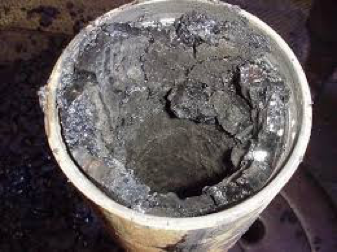
\includegraphics[width=0.45\linewidth]{clogged_pipe.png}}
\caption{Deposition of asphaltenes inside of a pipe \cite{Andrew:2006aa}.}
\end{figure}

%----------------------------------------------------------------------------------------
%	MATERIALS AND METHODS
%----------------------------------------------------------------------------------------

\begin{block}{Materials and Methods}

\begin{figure}
\fbox{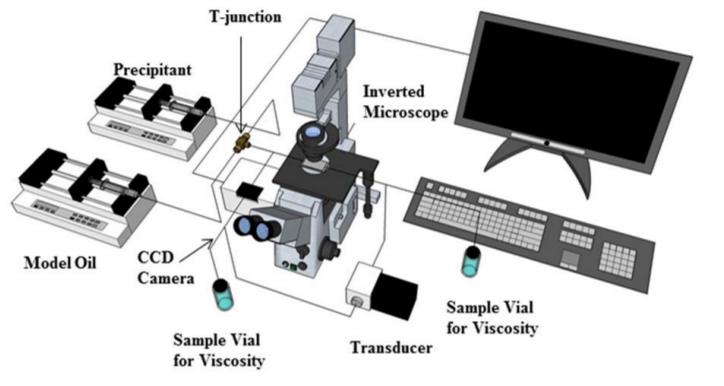
\includegraphics[width=0.9\linewidth]{materials.png}}
\caption{Experimental setup \cite{Lin:2016aa}.}
\end{figure}

\begin{enumerate}
\item Heptane and crude oil are pumped into the microfluidic device.
\item The pressure is recorded using a transducer.
\item Asphaltene deposition is recorded and measured using high speed optical microscopy.
\end{enumerate}

\end{block}

%---------------------------------------------------------------------

\end{column}						% End of the first column

\begin{column}{\sepwid}\end{column}	% Empty spacer column
\begin{column}{\twocolwid}			% Begin a column which is two columns wide (column 2)
\begin{columns}[t,totalwidth=\twocolwid]	% Split up the two columns wide column
\begin{column}{\onecolwid}\vspace{-.6in}	% The first column within column 2 (column 2.1)

%----------------------------------------------------------------------------------------
%	WATER'S IMPACT
%----------------------------------------------------------------------------------------

\begin{block}{Water's Impact on Deposition}

The presence of water in crude oil positively correlates with the deposition of asphaltenes and emulsions.

\vspace{1em}

\begin{figure}[!tbp]
  \centering
  \subfloat{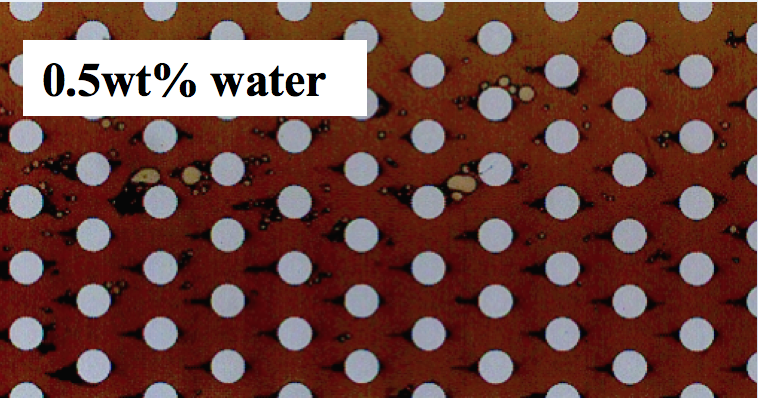
\includegraphics[width=0.55\textwidth]{05wt.png}}
  \hfill
  \subfloat{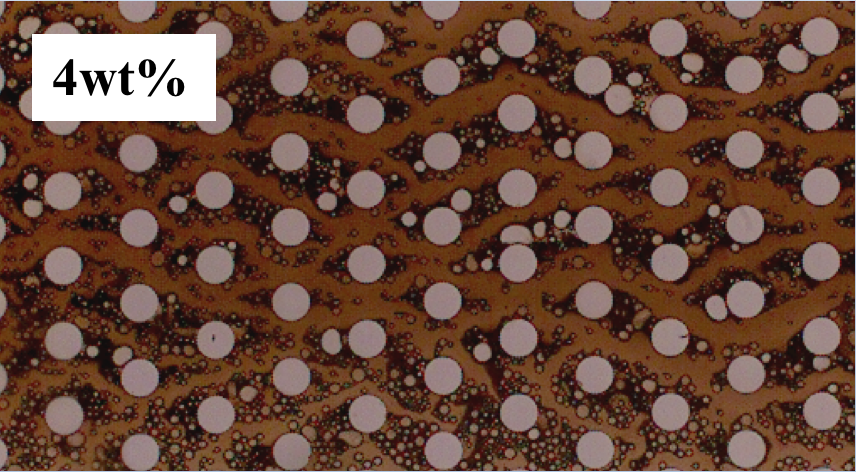
\includegraphics[width=0.55\textwidth]{4wt.png}} \\
  
  \subfloat{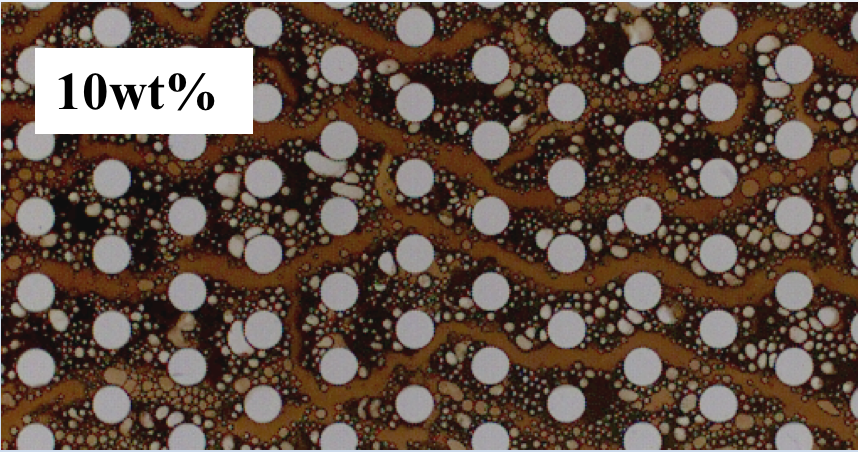
\includegraphics[width=0.55\textwidth]{10wt.png}}
  \hfill
  \subfloat{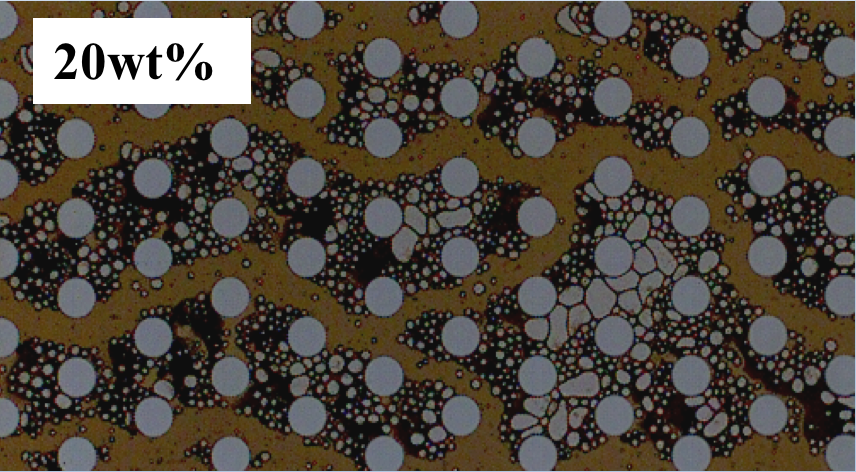
\includegraphics[width=0.55\textwidth]{20wt.png}}
  \caption{Asphaltene deposition inside the porous media with varying water concentrations. Courtesy of Yu-Jiun ``Nate'' Lin.}
\end{figure}

%\vspace{6.5em}

\centerline{\large{Water-in-Oil Emulsion Interface}}
\vspace{0.5em}
\begin{figure}
\fbox{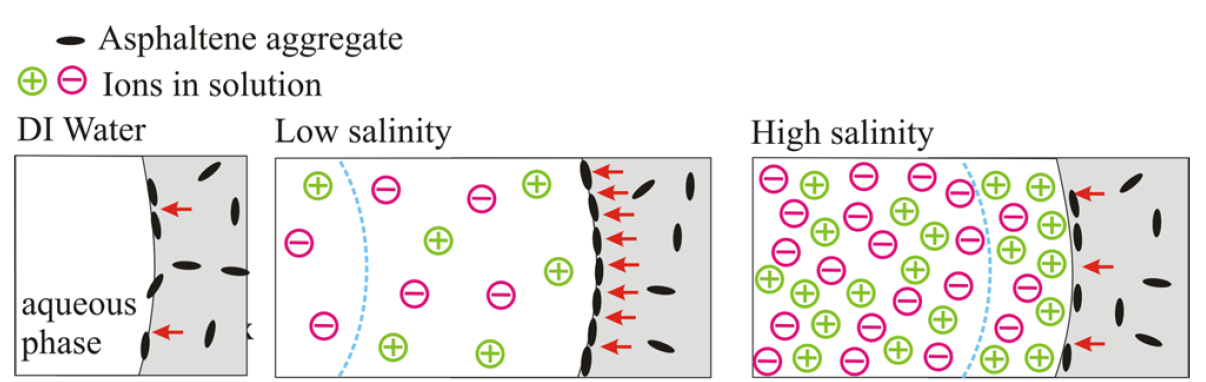
\includegraphics[width=0.8\linewidth]{emulsion_interface.png}}
\caption{The water-in-oil emulsion interface. T. Ch�vez-Miyauchi, et al. (2016).}
\end{figure}

The presence of salts disrupts the emulsion interface by introducing positive and negative ions that repel the asphaltenes from aggregating on the emulsion interface.

\end{block}

%----------------------------------------------------------------------------------------

\end{column} % End of column 2.1

\begin{column}{\onecolwid}\vspace{-.6in} % The second column within column 2 (column 2.2)

%----------------------------------------------------------------------------------------
%	SALT'S EFFECT
%----------------------------------------------------------------------------------------

\begin{block}{Salt's Impact on Deposition}

\begin{figure}
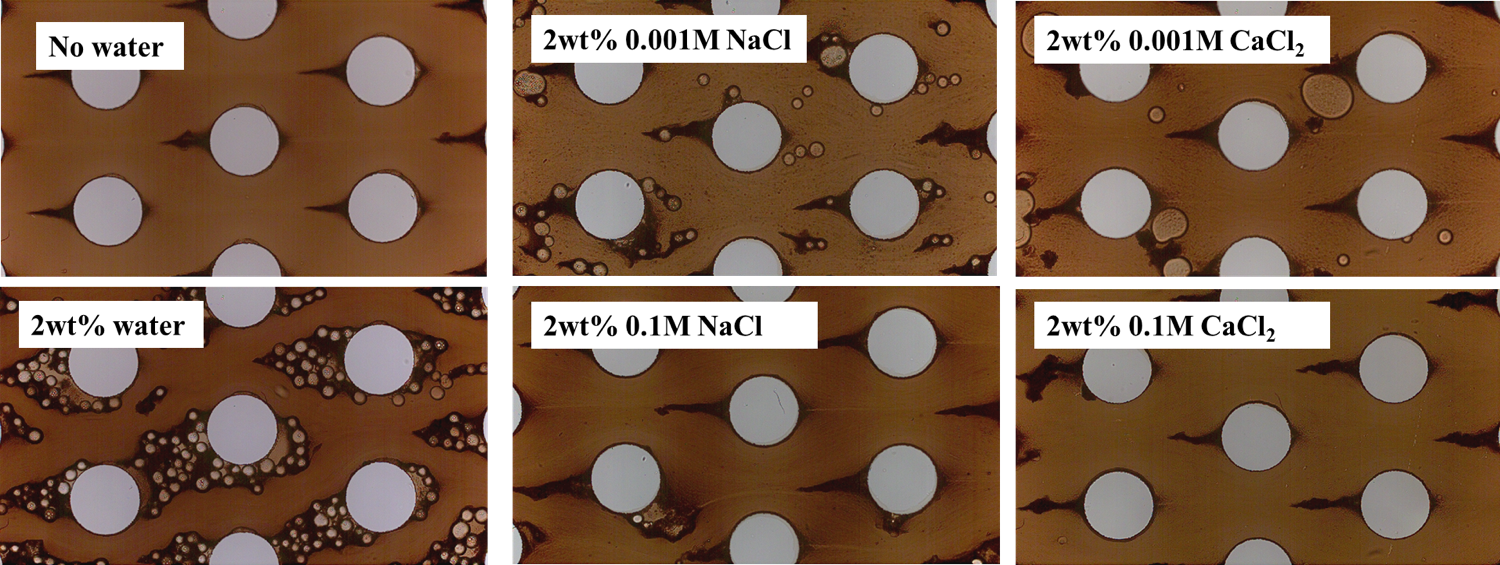
\includegraphics[width=0.8\linewidth]{salts.png}
\caption{Asphaltene deposition inside the porous media. These figures used a solution with 2 wt\% water. Each data set represents a specific concentration of sodium. Courtesy of Yu-Jiun ``Nate'' Lin.}
\end{figure}

\begin{figure}
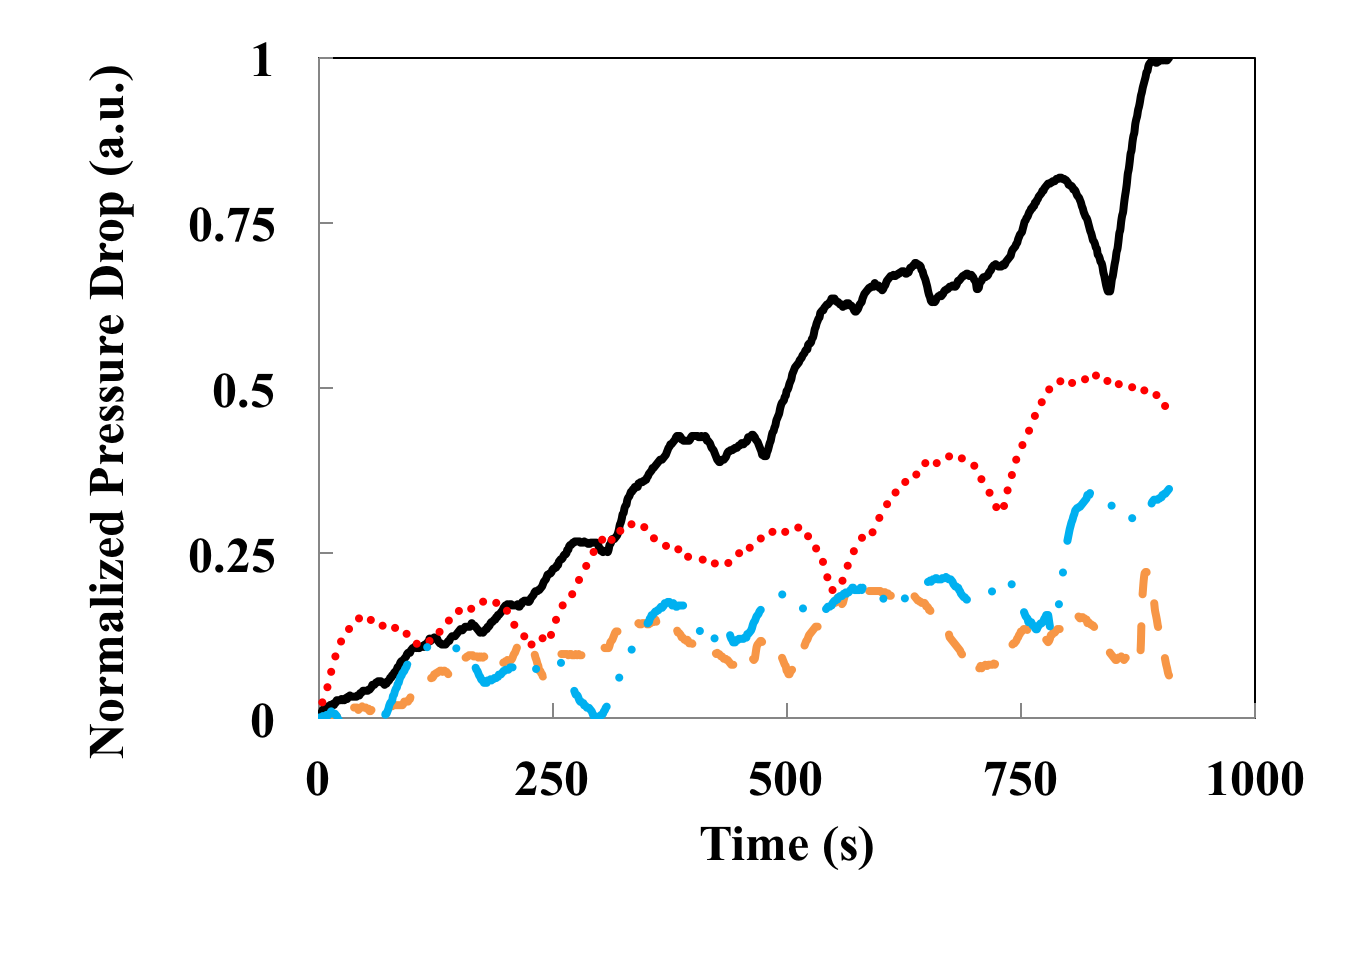
\includegraphics[width=0.9\linewidth]{2wt_salts.png}
\caption{The difference in pressure between the inlet and outlet of the microfluidics device. This figure used a solution with 2 wt\% water. Each data set represents a specific concentration of sodium. Courtesy of Yu-Jiun ``Nate'' Lin.}
\end{figure}

\begin{figure}
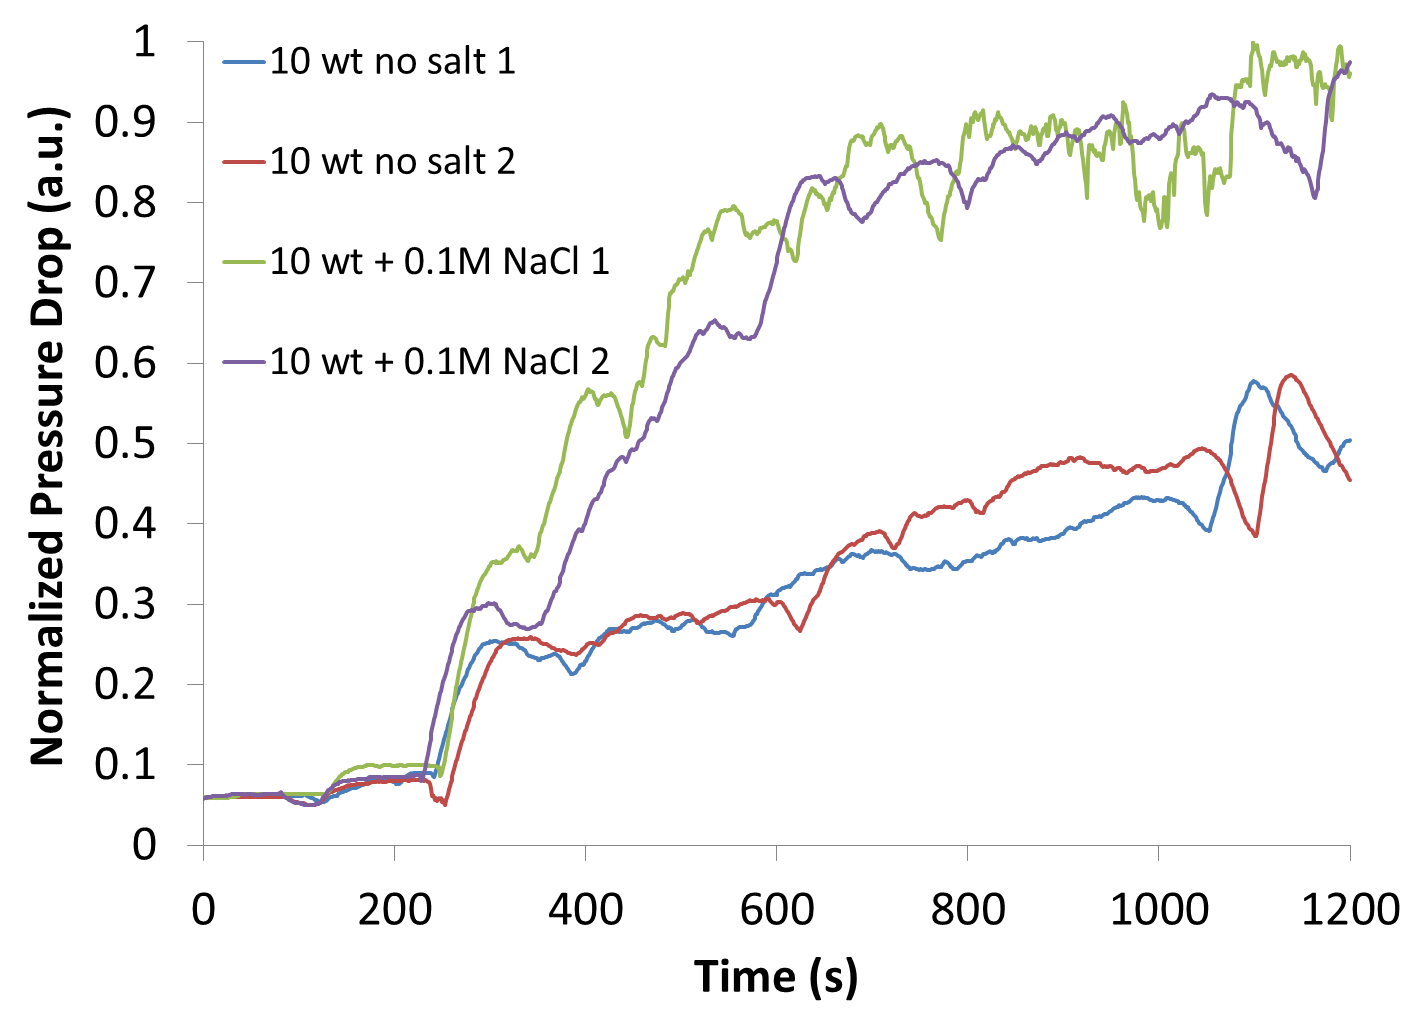
\includegraphics[width=0.9\linewidth]{10wt_salts.png}
\caption{The difference in pressure between the inlet and outlet of the microfluidics device. This figure used a solution with 10 wt\% water. Each data set represents a specific concentration of sodium.}
\end{figure}

\end{block}

%----------------------------------------------------------------------------------------

\end{column}	% End of column 2.2
\end{columns}	% End of the split of column 2 - any content after this will now take up 2 columns width
\end{column}	% End of the second column

\begin{column}{\sepwid}\end{column} % Empty spacer column
\begin{column}{\onecolwid} 		  % The third column

%----------------------------------------------------------------------------------------
%	CONCLUSION
%----------------------------------------------------------------------------------------

\begin{block}{Conclusion}

\textcolor{complement}{\textbf{The presence of water}} increases deposition by
\begin{itemize}
\item Aggregating with existing asphaltene depositions.
\item Clogging the flow streams and creating blockage.
\end{itemize}

\vspace{1em}

\textcolor{complement}{\textbf{The presence of salts}}
\begin{itemize}
\item Reduces the asphaltenes on the emulsion interface, but this effect is not linear.
\item Adding more salt causes smaller emulsions to come together and coalesce into bigger emulsions.
\item This increases blockage in the porous media.
\end{itemize}


\end{block}

%----------------------------------------------------------------------------------------
%	ACKNOWLEDGEMENTS
%----------------------------------------------------------------------------------------

\begin{block}{Acknowledgements}
Thank you to my mentors Peng and Nate, as well as my fellow undergraduate intern Sang for all of their patience and hard work training me in this field of study.

\vspace{1em}

This work is supported by the National Science Foundation under grant no. EEC-1461248.
\end{block}

%----------------------------------------------------------------------------------------
%	REFERENCES
%----------------------------------------------------------------------------------------

\begin{block}{References}

\nocite{*} % Insert publications even if they are not cited in the poster
\small{\bibliographystyle{unsrt}
\bibliography{sample}}

\end{block}

%----------------------------------------------------------------------------------------
%	CONTACT INFORMATION
%----------------------------------------------------------------------------------------

% \setbeamercolor{block alerted title}{fg=black,bg=norange} % Change the alert block title colors
% \setbeamercolor{block alerted body}{fg=black,bg=white} % Change the alert block body colors
\begin{comment}
\begin{block}{Contact Information}

\begin{itemize}
\item Email: hgducharme@gmail.com
\end{itemize}

\end{block}
\end{comment}

\vspace{3em}
\begin{center}
\begin{tabular}{ccc}
\fbox{
\includegraphics[width=0.7\linewidth]{RiceSTEM3.jpg}} & \hfill & \fbox{
\includegraphics[width=0.25\linewidth]{nsf1.png}}
\end{tabular}
\end{center}

%----------------------------------------------------------------------------------------

\end{column} % End of the third column

\end{columns} % End of all the columns in the poster

\end{frame}
\end{document}
